\documentclass[12pt]{extarticle}

\usepackage[utf8]{inputenc}
\usepackage[T1]{fontenc}
\usepackage{lmodern}
\usepackage{graphicx}
\usepackage{color}
\usepackage{hyperref}
\usepackage{amsmath}
\usepackage{amsfonts}
\usepackage{epstopdf}
\usepackage[table]{xcolor}
\usepackage[a4paper, total={6in, 10in}]{geometry}
\usepackage{enumitem}
\usepackage[export]{adjustbox}
\usepackage{algorithm2e}

\graphicspath{ {./Figures/} }



\begin{document}

{\Large Andrew Sivaprakasam | Warm-Up 1 Write-up}

GitHub Repo: \url{https://github.com/sivaprakasaman/Numerical_Methods_BME/} 

\section{Divide-and-Conquer for Integer Multiplication}
After implementing the provided \verb|multiply| algorithm, correctness was verified using the provided multiplications. 
\vspace{4pt}

Furthermore, runtime analysis was conducted, and no visible trend was observed, even after 10,000 repetitions of the given square product computations from 1,000 to 50,000. This may have been due to variations caused by the functions used to convert binary to decimal \verb|bin2dec| and \verb|dec2bin| or an implementation issue. 

\vspace{4pt}
The Master Theorem states that in a problem where \textit{a} subproblems of size $n/b$ that combines these subproblems with $O(n^d)$ time-complexity, the final time complexity will be $O(n^{log_b(a)})$ if $d < log_b(a)$. This is the case in the \verb|multiply| function since $log_2(3) \approx 1.6$.

\vspace{4pt}
I plotted this trend as a function of $N$ alongside the actual runtimes. Unfortunately, there does not appear to be a correlation in the two.
\vspace{12pt}

\begin{center}
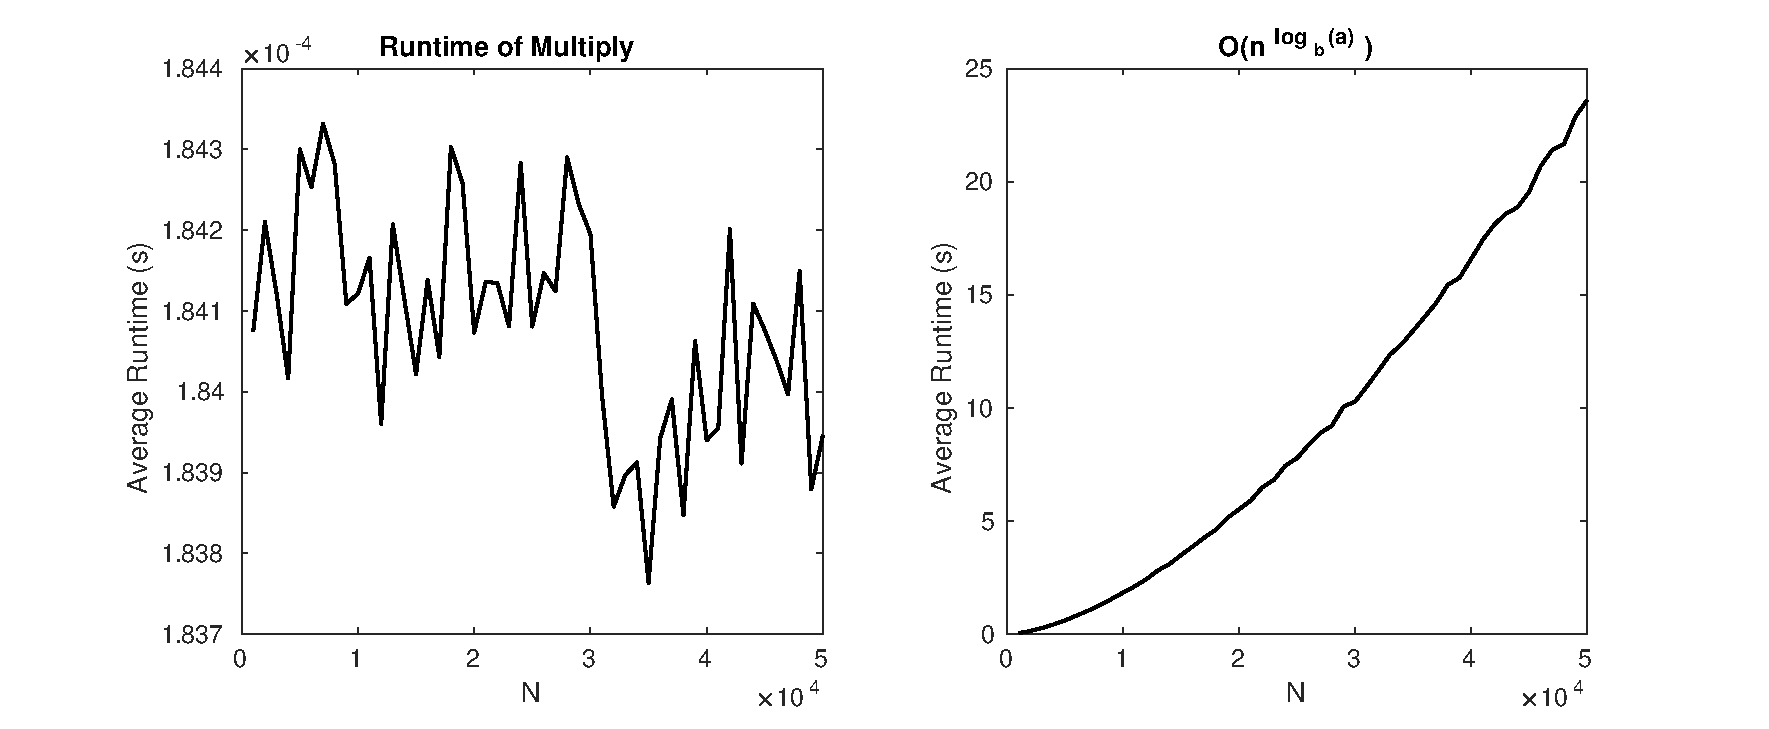
\includegraphics[width = 1.0\textwidth]{part1}\\
\vspace{12pt}
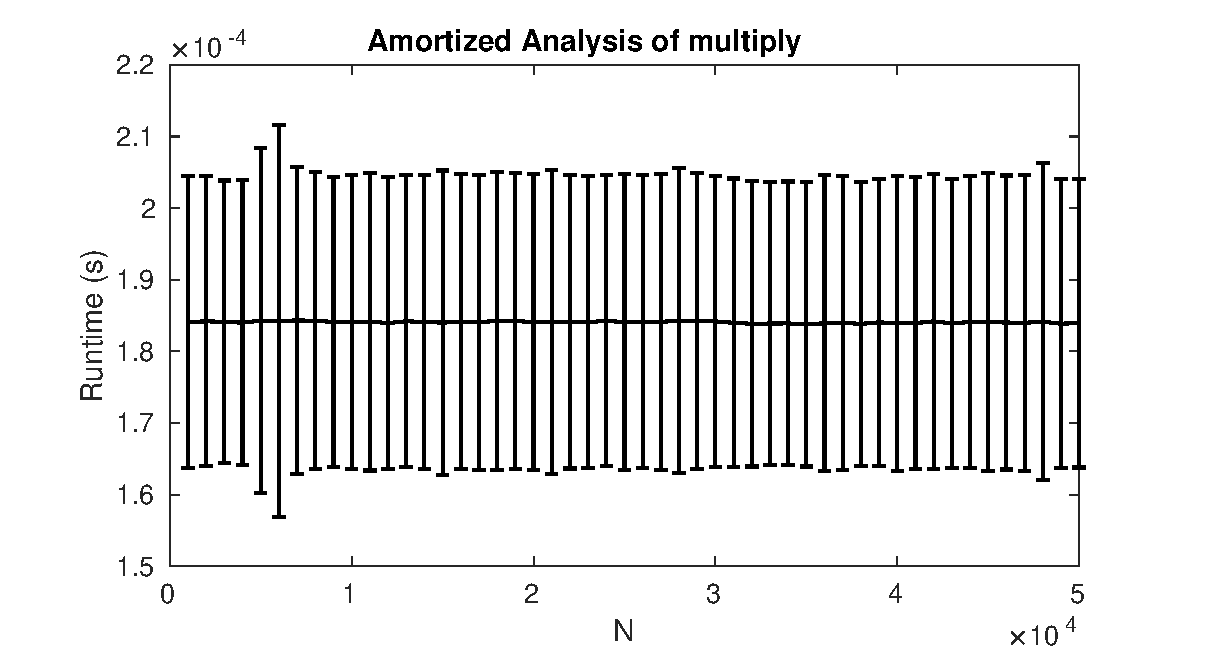
\includegraphics[width = .75\textwidth]{part1b}
\end{center}

\newpage
\section{Sorting Algorithms}
\subsection{Typset Sorting Algorithm Statements}
\textbf{Note: } My typset algorithms are \textit{zero-based}-- they assume indexing starts at zero, not the case in Matlab.

\vspace{12pt}
\hrule
\vspace{6pt}

\small\textbf{Bubble Sort:} Typset Algorithm. Worst/Average Case = $O(n^2)$, Best Case = $O(n)$ 
\vspace{6pt}
\hrule

\begin{algorithm}[H]
\SetKwInOut{Input}{input}\SetKwInOut{Output}{output}

\underline{function bubbleSort}($a[1,...,k]$)

\vspace{6pt}
\Input{An unsorted array, $a$}
\Output{The sorted array}
\BlankLine
\emph{Iterate through each element $i$ in $a$, swapping it with the element prior if element i-1 is greater than element i}
\BlankLine
swapped = \textbf{true}\;
\BlankLine
\While{swapped}{
	\BlankLine
	swapped = \textbf{false}\;
	\For{$i\leftarrow$ 1 \KwTo $k$-1}{
		\BlankLine
		\If{$a[i-1]>a[i]$}{swap: $a[i-1] \leftrightarrow a[i]$\;
		swapped = \textbf{true}\;}
		
	
	}

}
\vspace{6pt}
\end{algorithm}
\vspace{12pt}
\hrule
\vspace{6pt}
\textbf{Insertion Sort:} Typset Algorithm. Worst/Average Case = $O(n^2)$, Best Case = $O(n)$ 
\vspace{6pt}
\hrule

\begin{algorithm}[H]
\SetKwInOut{Input}{input}\SetKwInOut{Output}{output}
\underline{function insertionSort}($a[1,...,k]$)

\Input{An unsorted array, $a$}
\Output{The sorted array}
\vspace{6pt}

\emph{Incrementally traverse through each element $i$ in $a$, sliding $a[i]$ left through the sorted array, until it is ranked appropriately}
\vspace{6pt}\\
$i$ = 1\;
\vspace{6pt}

\While{$i$ < $k$}{
\vspace{6pt}
	$j$ = $i$\;
	\While{$j>0$ and $a[j-1]>a[j]$}{
		\vspace{6pt}
		swap: $a[j] \leftrightarrow a[j-1]$\;
		$j\leftarrow$ j - 1\;
	}	
	$i\leftarrow$ $i$ + 1\;
}
\end{algorithm}

\newpage
\vspace{6pt}
\hrule
\vspace{6pt}
\small\textbf{Selection Sort:} Typset Algorithm. Worst/Average/Best Case = $O(n^2)$ 
\vspace{6pt}
\hrule

\begin{algorithm}[H]
\SetKwInOut{Input}{input}\SetKwInOut{Output}{output}
\underline{function selectionSort}($a[1,...,k]$)

\Input{An unsorted array, $a$}
\Output{The sorted array}
\vspace{6pt}

\For{$i\leftarrow$ 0 \KwTo $k$-1}{
	\vspace{6pt}
	\emph{starting with element $i$, compare $i$ against elements ahead. If there is a new minimum, swap it with element $i$}	
		\vspace{6pt}

	tempMin = $i$\;	
	
	\BlankLine
	\For{$j\leftarrow i + 1$ \KwTo $k$}{
		\If{$a[j] < a[$tempMin$]$}{			
			tempMin = $j$\;
		}	
	}
	\vspace{6pt}
	\If{tempMin does not equal $i$}{
		swap: $a[i] \leftrightarrow a[$tempMin$]$\;
	}
}


\end{algorithm}

\subsection{Time and Space Complexity Justification}
\begin{center}
\includegraphics[width = .75\textwidth]{complexities}\\
\end{center}
\textbf{Time Complexity:}
\vspace{6pt}

Bubble Sort and Insertion Sort are the same in terms of their best, average, and worst-case time complexities. Both algorithms allow a single pass of iterations through every element in the array in the best case (already sorted array), $\Omega(n)$. In the average and worst cases for these algorithms, there will need to be some-sort of re-iteration through the array to accommodate out-of-order elements.\\ 

Selection Sort technically has worse best-case time-complexity than both Bubble Sort and Insertion Sort, because it requires a nested iteration, even in an already sorted array. Merge Sort has the best average and worst-case time complexities, since its recursive nature allows for solving of smaller sub-problems, to get to $O(nlog(n))$. However, its best case time-complexity is still worse than Bubble/Insertion sort because it does not change its necessary iterations even in a sorted array. 
\vspace{12pt}\\
\textbf{Space Complexity:}
\vspace{6pt}

Bubble, Insertion, and Selection Sort all have space complexity of $O(1)$, because the only additional space needed their operations is the storage of a single element to be swapped. Merge sort, however, has space complexity of $O(n)$ because it requires $N$ elements of storage as it breaks up the array into smaller arrays to sort and merge together. 
\\
\\
\textbf{*Note: }Time-complexity does not always translate to efficiency, since the number of elements swapped is not accounted for. Though Bubble Sort, Insertion Sort, and Selection Sort have the same or similar time-complexities, the number of swaps will be higher in Bubble Sort, decreasing its efficiency. 

\subsection{Experimental Testing of Amortized Analysis}

The aforementioned sorting algorithms were implemented in Matlab, and the runtimes were measured. Bubble Sort, though slightly lower in best-case time-complexity than Selection and Insertion Sort, performed worse than those two, presumably due to the inefficiency in the necessary number of swaps occuring during sorting. 
\\ \\
Additionally, Merge Sort did not perform as expected. It should have been the fastest of the implemented algorithms. \textit{This may be due to an implementation issue or a Matlab issue. }
\\ \\
Two additional sets of 10 arrays (dim = 500 and 100) were generated to further assess the runtimes.
\begin{center}
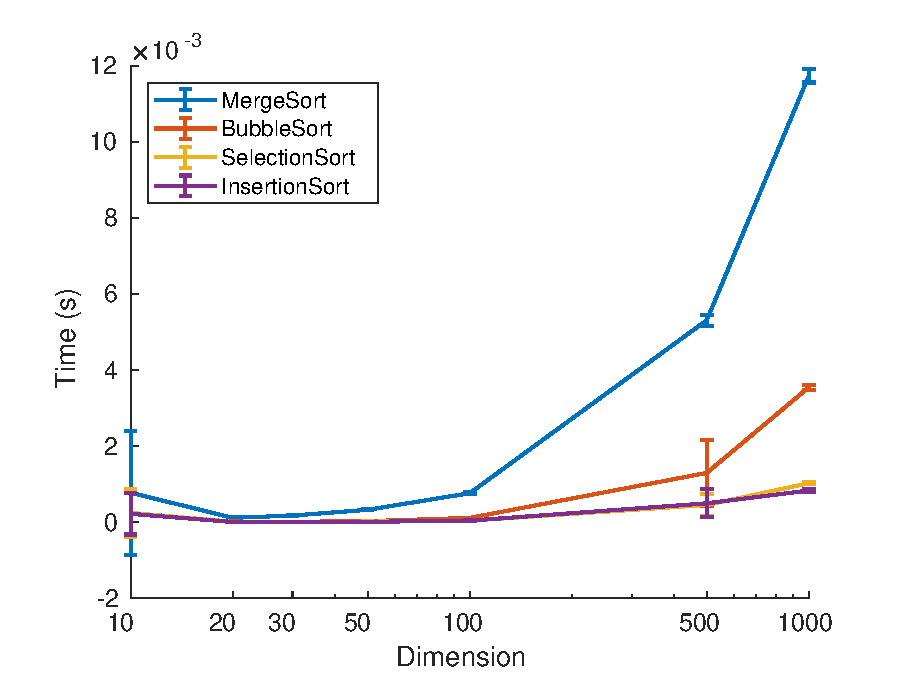
\includegraphics[width = .8\textwidth]{part2}
\end{center}
\end{document}